%In dit hoofdstuk moet het volgende besproken worden:
%-Uitleggen van het probleem
%-Hoe ik tewerk ga gaan
%-Gaan we concluderen met de onderzoeksvraag
\chapter{Inleiding}\label{hfdst:situering}
\section{Situering}
%%% TODO meer schrijven over wat televic rail doet en wat zij maken -> uitleggen dat framework daarbij te pas komt
%http://www.railway-technology.com/contractors/operation/televic-rail/
Met meer dan 30 jaar ervaring in het ontwerpen en onderhouden van on-board communicatiesystemen is Televic Rail een toonaangevende producent van Passenger Information Systems, Entertainment Systems and Infotainment Systems.
LiveCom is Televic Rail nieuwste generatie van informatie management systemen.
Het integreert van alle aspecten van de on- en off-board reizigersinformatie, infotainment en entertainment. 
Het stelt operatoren in staan om hun volledige verkeersschema's, dienstregelingen, routes, stations en alles met betrekking tot informatie en infotainment omtrent passagiers te beheren, met behulp van off-board software tools.

iCoM, de geïntegreerde oplossing van Televic Rail voor passagiersgegevens en communicatiemanagement, biedt het openbaar vervoer en spoorwegondernemingen een centraal systeem voor het creëren, het beheren, het distribueren en het uitvoeren van real-time on en off-board generieke en commerciële passagiersinformatie op de vloot, in stations en bij haltes.

Naast deze systemen heeft Televic verschillende mechatronica-sensoren en veiligheidcontrolesystemen ontworpen.
Alle systemen en apparaten zijn ontworpen in overeenstemming met de betreffende spoorwegsectornormen en voldoen aan de eisen voor passagiersruimte, draaistel en asmontage. 
On-board controllers verwerken sensordata-informatie en sturen deze naar de betreffende actuators en treinbeheersingssystemen.
Fysische parameters die momenteel worden ondersteund zijn onder andere versnelling, druk, rotatie, temperatuur, geluid en de verplaatsing.

Om te voldoen aan de strenge veiligheidsnormen heeft Televic Rail een Python test framework ontworpen waarmee Televic in staat is om verschillende producten te onderwerpen aan verschillende testscenario's.
Het framework werd ontworpen om gebruikt te worden op verschillende testtorens en werd later aangepast om bruikbaar te zijn op gewone computers.
Dit framework wordt intensief gebruikt tijdens het productieproces en is cruciaal voor het afleveren van producten die voldoen aan de strenge veiligheidsnormen.

%%% TODO schetsen van structuur van het framework

\section{Probleemstelling}\label{sec:probleem}
Het Python testraamwerk moet correct functioneren met een grote hoeveelheid aan producten die Televic fabriceert.
Hierdoor gebruikt het Python testraamwerk verschillende drivers en bibliotheken.
Een direct gevolg hiervan is dat het installatieproces tijdrovend en foutgevoelig is.
Verder dient elk nieuw toestel op het raamwerk ondersteunt te worden waardoor er jaarlijks ettelijke releases van het raamwerk verspreid worden.
Het installatieproces en updateproces vragen om een vereenvoudiging zodat het testraamwerk gebruiksvriendelijker wordt.

Doordat het installatieproces en updateproces foutgevoelig zijn, moet een rampenplan voorzien worden.
Door de aanwezigheid van een rampenplan, worden mogelijke fouten vermeden en indien nodig opgevangen en verholpen.
Zo wordt vermeden dat de productielijn moet worden stilgelegd door bijvoorbeeld een fout tijdens het updaten van het testraamwerk.
Het is dus belangrijk dat het testraamwerk op een eenvoudige manier geïnstalleerd en geüpdatet kan worden op verschillende testtorens.
Om dit te laten slagen moet het testraamwerk eerst bij de verschillende testtorens geraken.
Er zullen dus producenten van software zijn die de verschillende testraamwerken produceren en willen verspreiden maar ook gebruikers die deze willen ontvangen.
Het proces waar bij software van een producent naar alle toepasbare gebruikers wordt verspreid en vervolgens geïnstalleerd wordt, wordt ook wel het deployment proces genoemd.
Een kleine schets van dit idee is zichtbaar in Figuur~\vref{fig:simpleServerClient}.

\begin{figure}[!ht]
\centering
\makebox[0pt]{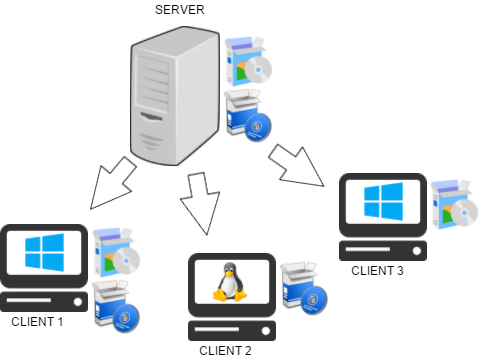
\includegraphics[scale=0.7]{afbeelding/simpelServerClient.png}}
\caption{Voorstelling van software verspreiding}
\label{fig:simpleServerClient}
\end{figure}

Tijdens het zoeken naar een oplossing voor het installatieproces en updateproces van het Python testraamwerk, moet gezocht worden naar een oplossing die ook antwoorden biedt op toekomstige problemen.
Tot op heden werd ervan uitgegaan dat de enige applicatie die verspreid, geïnstalleerd en geüpdatet moet worden het Python testraamwerk is.
In de toekomst moet het evenwel mogelijk zijn om verschillende applicaties van Televic te ondersteunen.
Het is dan ook belangrijk dat een oplossing gevonden wordt die een groeiend aantal gebruikers ondersteunt.
Naargelang het aantal applicaties die ondersteunt worden stijgt, zullen meer systemen gebruik maken van de applicatie.
Naarmate het aantal gebruikers stijgt, stijgt ook de vraag naar een algemene administratieve interface.
Verschillende versies van de applicaties zullen in omloop zijn waardoor de nood aan een administratieve interface stijgt. 
Met een administratie interface wordt het mogelijk om bij te houden hoe het uitrollen van een nieuwe versie van het testraamwerk verloopt maar naar de toekomst toe zou het mogelijk moeten zijn om verschillende gebruikers bij te staan.
Deze informatie kan gebruikt worden om het verspreidingsproces bij te sturen zodat een volgende keer het proces vlotter verloopt.
Naast het ondersteunen van verschillende applicatie moet tijdens het ontwerpen rekening gehouden worden met verscheidene besturingssystemen.
Huidige systemen draaien op Windows maar het gebruik van Linux is in de toekomst niet uit te sluiten.

Het doel van deze thesis is dan ook een oplossing te vinden voor het complexe installatieproces en updateproces.
Daarbij moet de software eerst van de producent bij de gebruikers geraken en moeten deze processen rekening houden met een rampenplan om fouten tijdens een installatie of update op te vangen.
Verder wordt tijdens de ontwerpfase van de applicatie rekening gehouden met een groeiend aantal applicaties die verspreid en geïnstalleerd moeten worden, een groeiend aantal gebruikers die deze applicaties willen ontvangen en de diversiteit van besturingssystemen van deze gebruikers.

\section{Overzicht}
Het tweede hoofdstuk bevat een literatuurstudie over het probleem van Televic.
Er wordt nagegaan welke technologieën en architecturen beschikbaar zijn om ieder deelprobleem op te kunnen lossen.

Vervolgens vindt in het derde hoofdstuk een selectie plaats van de meest geschikte technologieën en architecturen.
De gekozen technologieën worden gecombineerd tot één solide architectuur die de basis vormt voor de implementatie.
Er worden verscheidene diagrammen ontworpen die gebruikt gaan worden tijdens het implementeren van de functionaliteiten.

In het vierde hoofdstuk worden de meeste Python modules overlopen en worden enkele implementatie keuzes verder toegelicht en uitgediept.

Het vijfde hoofdstuk wordt gebruikt om de ontworpen applicatie onderworpen aan verscheidene testscenario's om te achterhalen of de applicatie voldoet aan de verwachten.
Hierna volgt een SWOT analyse om na te gaan wat eventuele uitbreidingen maar ook zwaktes zijn van de applicatie.

